\documentclass[11pt,slovak,a4paper,usepdftitle=false]{article}

\usepackage[slovak]{babel}
\usepackage[T1]{fontenc}
\usepackage[utf8]{inputenc}
\usepackage{graphicx}
\usepackage{url} % \url
\usepackage{hyperref} % Automatic links
\usepackage{parskip}
\usepackage[left=2cm, right=2cm]{geometry}
\usepackage{listings}
\usepackage{xcolor}
\usepackage{amsmath}
\usepackage{placeins}
\usepackage{cite}
\usepackage{listings}
\usepackage{xcolor}
\usepackage{pgfkeys}
\usepackage{pdfpages}
\usepackage{tabto}
\usepackage{enumitem}
\usepackage{longtable}

\newcommand{\spc}{\,}

\setlist{itemsep=0.4em, parsep=0em, midpenalty=3000}

\hypersetup{pdftitle=Generátor plošinových hier,pdfdisplaydoctitle}

\pgfkeys{
    /codeblock/.is family, /codeblock,
    default/.style = {start = 1, end = 1, language=None},
    start/.estore in = \codeblockStart,
    end/.estore in = \codeblockEnd,
    language/.estore in = \codeblockLanguage,
}
\newcommand\codeblock[2][]{\pgfkeys{/codeblock, default, #1}\lstinputlisting[firstnumber=\codeblockStart,firstline=\codeblockStart,lastline=\codeblockEnd,language=\codeblockLanguage]{#2}}

\definecolor{codegreen}{rgb}{0,0.6,0}
\definecolor{codegray}{rgb}{0.5,0.5,0.5}
\definecolor{codedark}{rgb}{0.3,0.3,0.3}
\definecolor{codepurple}{rgb}{0.58,0,0.82}

\lstdefinestyle{mystyle}{ 
    %commentstyle=\sffamily\color{codegreen},
    commentstyle=\color{codegreen},
    keywordstyle=\color{magenta},
    numberstyle=\tiny\color{codegray},
    stringstyle=\color{codepurple},
    basicstyle=\ttfamily\footnotesize\color{codedark},
    breakatwhitespace=true,
    identifierstyle=\color{black},      
    breaklines=true,                 
    captionpos=b,                    
    keepspaces=true,                 
    numbers=left,                    
    numbersep=5pt,                  
    showspaces=false,                
    showstringspaces=false,
    showtabs=false,                  
    tabsize=4
}

\lstdefinelanguage{json}
{
    morestring=[b]",
    morestring=[d]'
}

\lstset{
	style=mystyle,
	inputencoding=utf8,
    columns=fullflexible,
	literate={ú}{{\'u}}1 {í}{{\'i}}1 {á}{{\'a}}1 {ĺ}{{\'l}}1 {é}{{\'e}}1 {ý}{{\'y}}1 {ó}{{\'o}}1 {ž}{{\v{z}}}1 {š}{{\v{s}}}1 {ď}{{\v{d}}}1 {č}{{\v{c}}}1 {ň}{{\v{n}}}1 {ť}{{\v{t}}}1 {ľ}{{\v{l}}}1 {ä}{{\"{a}}}1 {Δ}{{\ensuremath{\Delta}}}1
}

% definuje nadpis bez čísla, použitý pri prílohách
\newcommand{\usection}[1]{\section*{#1}
\addcontentsline{toc}{section}{#1}}

\DeclareUnicodeCharacter{21D2}{\ensuremath{\Rightarrow}}

\renewcommand{\familydefault}{\sfdefault} % Sans serif
\raggedright

% použiť hiearchiálne ordered lists
\renewcommand{\labelenumii}{\theenumii}
\renewcommand{\theenumii}{\theenumi.\arabic{enumii}.}

\renewcommand{\labelenumiii}{\theenumiii}
\renewcommand{\theenumiii}{\theenumii\arabic{enumiii}.}

\renewcommand{\labelenumiv}{\theenumiv}
\renewcommand{\theenumiv}{\theenumiii\arabic{enumiv}.}

\pagestyle{plain}
\pagenumbering{roman}

\begin{document}


\includepdf[pages=-]{ref-title-page.pdf}

% zadná strana titulného listu (prázdna strana)
\null \thispagestyle{empty}

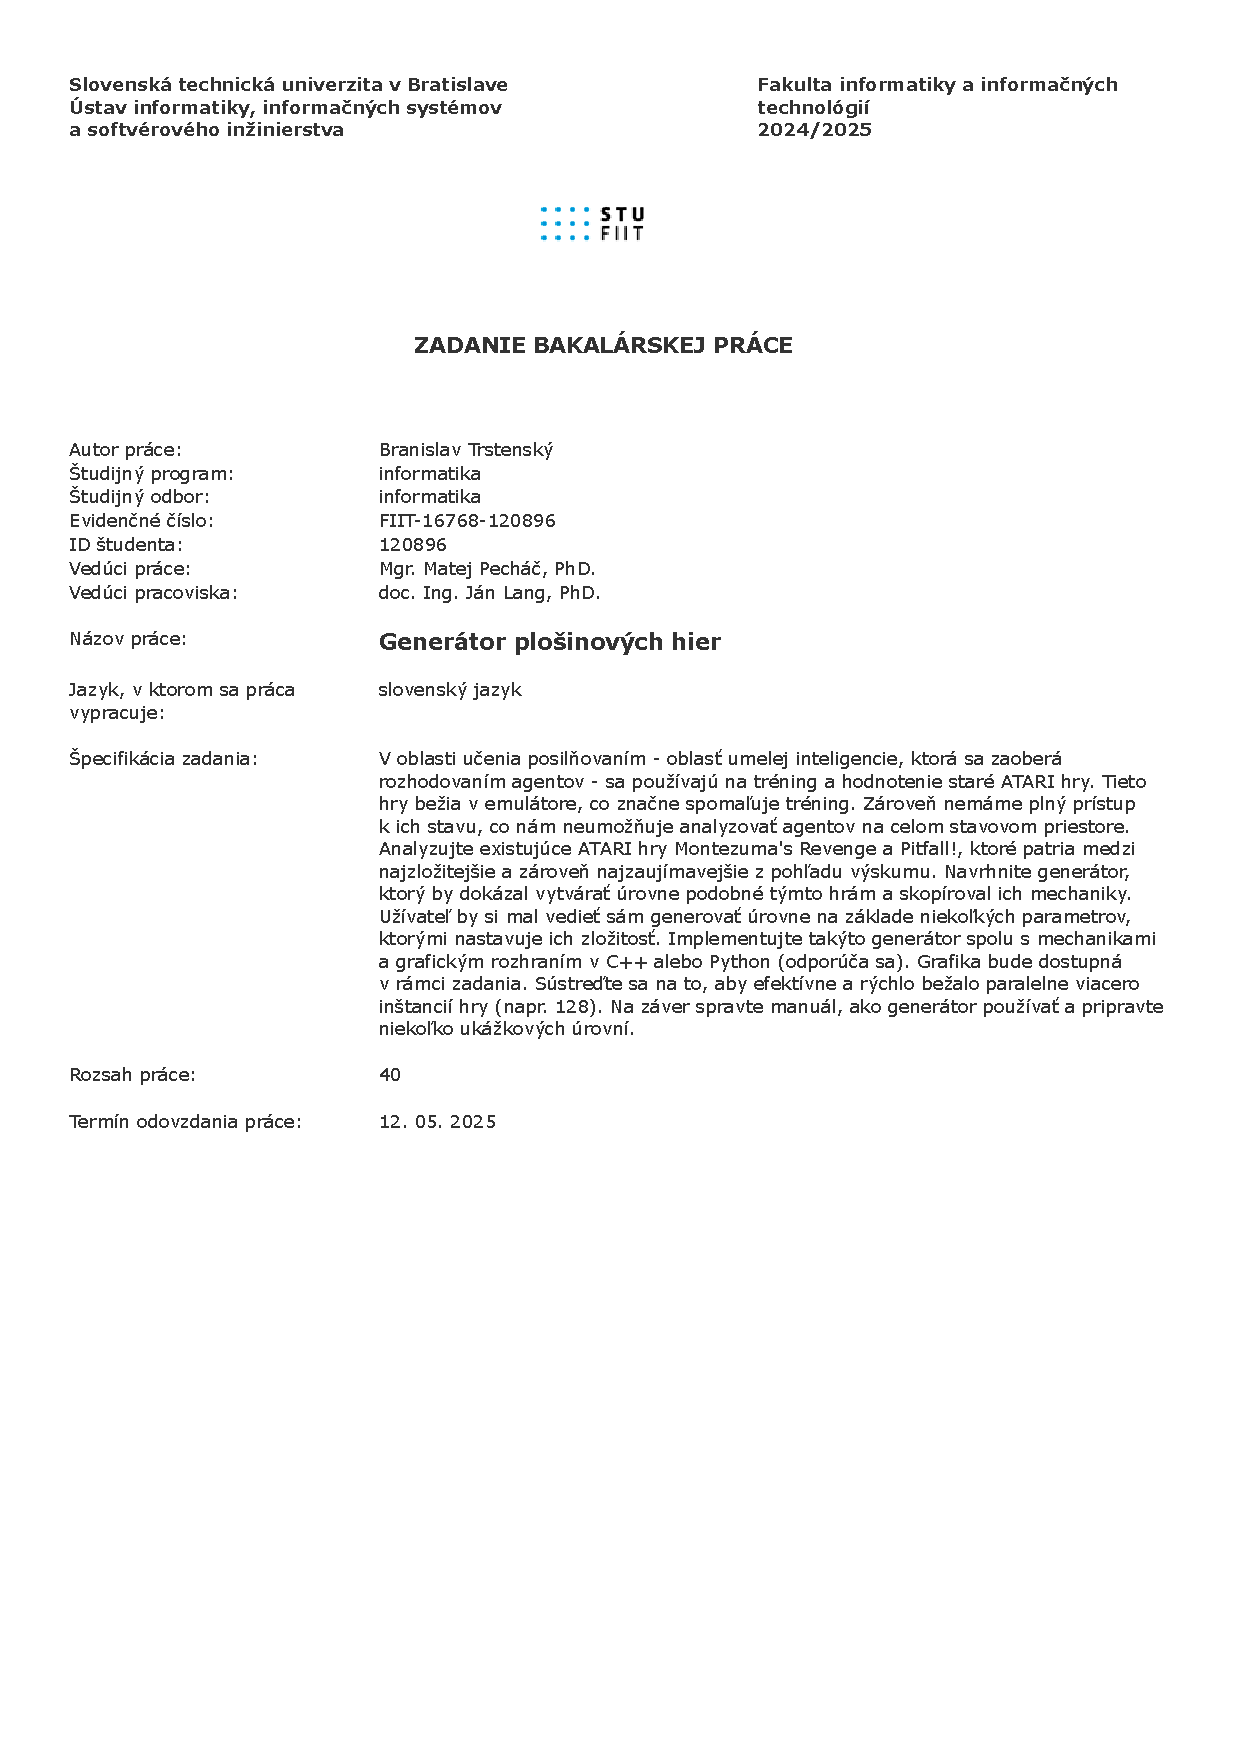
\includepdf[pages=-]{ref-zadanie.pdf}

% zadná strana zadania/revízie (môže byť prázdna)
\null \thispagestyle{empty}

\newpage

% čestné vyhlásenie je napísané na spodku strany
\null \thispagestyle{empty} \vfill

Čestne vyhlasujem, že som túto prácu vypracoval(a) samostatne, na základe konzultácií
a s použitím uvedenej literatúry.

V Bratislave, \today.

\begin{flushright}
    Branislav Trstenský
\end{flushright}

\newpage

% zadná strana čestného prehlásenia (prázdna strana)
\null \thispagestyle{empty}

\newpage

\section*{Anotácia}

Slovenská technická univerzita v Bratislave

FAKULTA INFORMATIKY A INFORMAČNÝCH TECHNOLÓGIÍ

\NumTabs{3}

Študijný program: \tab informatika

Autor: \tab Branislav Trstenský

Bakalárska práca: \tab Generátor plošinových hier

Vedúci diplomovej práce: \tab Mgr. Matej Pecháč, PhD.

Január 2025


Pri spätnoväzobovom učení, v oblasti umelej inteligencie zaoberajúcej sa rozhodovaním agentov, sa používajú na tréning a hodnotenie staré ATARI hry. Tieto hry bežia v emulátore, čo značne spomaľuje tréning. Zároveň nemáme plný prístup k ich stavu, čo nám neumožnuje analyzovať agentov na celom stavovom priestore. 

Táto práca sa zaoberá vytvorením generátora, ktorý je schopný vytvoriť úrovne podobné ATARI hrám,  ako sú Pitfall! alebo Montezuma's Revenge, ktoré patria medzi najzložitejšie a zároveň najzaujímavejšie z pohľadu výskumu.

Generátor umožňuje používateľovi jednoducho vytvoriť nové úrovne nastavením malého počtu parametrov. Tiež je jeho súčasťou replikácia mechaník týchto hier, čo umožňuje tieto hry spustiť pre použitie s agentom umelej inteligencie.

\newpage

% zadná strana anotácie (prázdna strana)
\null \thispagestyle{empty}

\newpage

\section*{Annotation}

Slovak University of Technology Bratislava

FACULTY OF INFORMATICS AND INFORMATION TECHNOLOGIES

\NumTabs{3}

Degree course: \tab informatika

Autor: \tab Branislav Trstenský

Bachelor's Thesis: \tab Platform game generator

Supervisor: \tab Mgr. Matej Pecháč, PhD.

Január 2025

For reinforcement learning, in the field of artificial intelligence dealing with agent decision-making, old ATARI games are used for training and evaluation. These games run in an emulator, which significantly slows down training. At the same time, we do not have full access to their state, which does not allow us to analyze agents in the entire state space.

This thesis deals with the creation of a generator capable of generating levels similar to ATARI games such as Pitfall! or Montezuma's Revenge, which are among the most complex and at the same time most interesting from a research point of view.

The generator allows users to easily create new levels by setting a small number of parameters. It also includes a replica of the mechanics of these games, which allows these games to be run for use with an artificial intelligence agent.

\newpage

% zadná strana anotácie (prázdna strana)
\null \thispagestyle{empty}

\newpage

\thispagestyle{plain}
\tableofcontents

\newpage

% posledná zadná strana obsahu (alebo zoznamov) (ak je prázdna, číslo strany sa neuvádza)
\null \thispagestyle{empty}

\newpage

\setcounter{page}{1}
\pagenumbering{arabic}

\widowpenalties 1 10000
\input{doc.tex}

\newpage

\Urlmuskip=0mu plus 1mu
\def\UrlBreaks{\do\/\do-}

\addcontentsline{toc}{section}{Literatúra}
\bibliography{bibliography}
\bibliographystyle{stn690}

\newpage

\usection{Príloha A: Návod k použitiu programu}

\subsection*{Použitie programu priamo}

Program potrebuje k svojej činnosti zdroje. Očakáva že bude mať k dispozíií priečinok \texttt{assets} umiestnený vo working directory. Zdroje sú uložené v globálnych objektoch ktoré treba načítať.

\begin{lstlisting}[language=python]
import pygame
from pg_gen.generation.RoomPrefabRegistry import RoomPrefabRegistry
from pg_gen.level_editor.ActorRegistry import ActorRegistry
from pg_gen.support.constants import ROOM_FOLDER

pygame.init()
ActorRegistry.load_actors()
RoomPrefabRegistry.load(ROOM_FOLDER)
\end{lstlisting}

Ďalším krokom je zvoliť si obtiažnosť ktorú vyžadujete. Parametre majú následovný výzam:

\begin{itemize}
    \item \texttt{JUMP} ⇒ počet skokov v ceste
    \item \texttt{REWARD} ⇒ počet drahokamov v ceste
    \item \texttt{ENEMY} ⇒ počet nepriateľov v ceste (obtiažnejší nepriateľia sa rátajú ako viacej nepriateľov)
    \item \texttt{SPRAWL} ⇒ dĺžka cesty
\end{itemize}

\begin{lstlisting}[language=python]
from pg_gen.generation.RoomParameter import UNUSED_PARAMETER
from pg_gen.difficulty.DifficultyReport import DifficultyReport

target_difficulty = DifficultyReport()
target_difficulty.set_all_parameters(UNUSED_PARAMETER)
target_difficulty.set_parameter(RoomParameter.REWARD, 500)
target_difficulty.set_parameter(RoomParameter.JUMP, 10)
target_difficulty.set_parameter(RoomParameter.ENEMY, 100)
target_difficulty.set_parameter(RoomParameter.SPRAWL, 50)
\end{lstlisting}



Následne je potrebné vytvoriť optimizátor, a vložiť do neho zvolené parametre. Optimizátor ďalej príjima argumenty \texttt{random}, kde je potrebné vložiť náhodný generátor - tu je možné nastaviť konsistetný seed. Optimizátor má možnosť nastaviť populáciu cez parameter \texttt{max\_population} a počet iterácií cez parameter \texttt{max\_generations}.

\begin{lstlisting}[language=python]
from random import Random
from pg_gen.game_core.Universe import Universe
from pg_gen.difficulty.DifficultyOptimizer import DifficultyOptimizer

universe = Universe()
optimizer = DifficultyOptimizer(universe, target_difficulty=target_difficulty, random=Random(108561))
\end{lstlisting}

Nie je potrebné špecifikovať všetky parametre, nepoužité parametre ostanú ako \texttt{UNUSED\_PARAMETER}. Tieto parametre budú mať po optimizácií náhodnú hodnotu, pravdepodobne je múdre ich nastaviť na konštatnú hodnotu. Takto je možné nastaviť všetky parametre, ktoré sa menia pri optimalzácií.

\begin{lstlisting}[language=python]
from pg_gen.generation.RoomParameter import RoomParameter

optimizer.get_parameter(RoomParameter.REWARD).override_value(0.5)
\end{lstlisting}

Po zvolení parametrov a obtiažnosti je možné spustiť optimizátor.

\begin{lstlisting}[language=python]
optimizer.initialize_population()
optimizer.optimize()
\end{lstlisting}

Po optimizácií je možné vybrať najbližšieho kandidáta a použiť jeho úroveň. Následne je potrebné aktivovať koreňovú miestnosť a vložiť do nej objekt hráča.

\begin{lstlisting}[language=python]
from pg_gen.generation.RoomController import RoomController
from pg_gen.actors.Player import Player
from pg_gen.support.Point import Point
from pg_gen.support.constants import ROOM_HEIGHT, ROOM_WIDTH

best_candidate = optimizer.get_best_candidate()
map = best_candidate.get_map()
universe.map = map

room_controller = RoomController.initialize_and_activate(universe, map.get_room(Point.ZERO), None)
room_controller.world.add_actor(Player(position=Point(ROOM_WIDTH / 2, ROOM_HEIGHT / 2)))
\end{lstlisting}

Pre použitie hry interaktívne stači spustiť \texttt{InteractiveGameLoop}.

\begin{lstlisting}[language=python]
from pg_gen.game_core.InteractiveGameLoop import InteractiveGameLoop

game_loop = InteractiveGameLoop(universe)
game_loop.run()
\end{lstlisting}

Pre použitie s modelom je potrebné vytvoriť vlastný pygame-ový \texttt{Surface} a vložiť ho do \texttt{GameLoop}. Následne je možné vkladať vstup cez objekt \texttt{InputState} a manuálne simulovať update. Keďže mimo interaktívneho prístupu nie je herná sluťka naviazaná na reálny čas, je potrebné stanoviť čas, ktorý prejde medzi každý update krokom. Napríklad: ak chceme mať 20 krokov cez jednu simulovanú sekundu, tak čas medzi krokmi je $ 1 / 20 $ sekúnd.

\begin{lstlisting}[language=python]
from pg_gen.game_core.GameLoop import GameLoop
from pg_gen.support.constants import CAMERA_SCALE
from pg_gen.game_core.InputState import InputState

surface = pygame.display.set_mode((CAMERA_SCALE * ROOM_WIDTH, CAMERA_SCALE * ROOM_HEIGHT))
self.game_loop = GameLoop(surface, self.universe)

input_state = self.universe.di.inject(InputState)
input_state.clear()

input_state.left = True
input_state.jump = True
# [...]

game_loop.update_and_render(1 / fps)
\end{lstlisting}

\subsection*{Použitie Gymnasium prostredia}

Gymnasium prostredie rieši spustenie hernej slučky automaticky. Stačí inicializovať globálne objekty a vložiť úroveň. Najskôr však treba registrovať prostredie do Gymnasia.

\begin{lstlisting}[language=python]
from gymnasium.envs.registration import register
from gymnasium_int.PgEnv import PgEnv

register(
    id="gymnasium_int/PgEnv",
    entry_point=PgEnv,
)
\end{lstlisting}

Následne je možné vytvoriť prostredie.

\begin{lstlisting}[language=python]
env = gymnasium.make("gymnasium_int/PgEnv", render_mode="rgb_array", level=level)
observation, info = env.reset()
\end{lstlisting}

Prostredie podporuje dva render módy:

\begin{itemize}
    \item \texttt{human} ⇒ simulácia prebieha v reálnom čase a je otvorené okno, kde je možné vidieť výstup z hry
    \item \texttt{rgb\_array} ⇒ simulácia prebieha najrýchlešie ako je možné, výstupom modelu je array obsahujúci grafický výstup hry
\end{itemize}

Pri použití \texttt{rgb\_array}, kedže sa neotovrí okno, je potrebné manuálne inicializovať grafický systém pygame-u. Najjednoduchší spôsob, ako toto dosiahnuť je vytvoriť jednopixelové skryté okno, ktoré nebude na nič využité.

\begin{lstlisting}[language=python]
if env.render_mode == "rgb_array":
    pygame.display.set_mode((1, 1), flags=pygame.HIDDEN)
\end{lstlisting}

Ako level je možné dodať:

\begin{itemize}
    \item string ⇒ ako explicitný názov miestnosti, ktorá bude vygenerovaná; toto je možné použiť pre testovanie konkrétnej mechaniky
    \item callback ⇒ funckia dostane ako argument referenciu na \texttt{Universe} a musí vrátiť \texttt{Map} objekt, vo funkcií spustite generáciu ako v predošlej sekcií
\end{itemize}

Toto je jednoduchý loop, pre využitie prostredia:

\begin{lstlisting}[language=python]
episode_over = False
while not episode_over:
    action = env.action_space.sample()
    observation, reward, terminated, truncated, info = env.step(action)

    episode_over = terminated or truncated
    print(action, observation, info, reward)

env.close()
\end{lstlisting}




\end{document}
